\chapter{De la Naturaleza al Temperamento}
\label{chap4}
Un piano y un violín son dos universos sonoros en esencia opuesta. Para producir sonido en un piano, se acciona una de sus teclas —blancas o negras—, lo que activa un martillo que golpea una cuerda en su interior. La nota resultante depende exclusivamente de la tensión, la densidad y la longitud de esa cuerda. Dado que estas magnitudes son inalterables durante la interpretación, cada tecla produce un sonido único e inmutable. Esto confina al piano a un paleta de sólo 88 sonidos discretos, y toda la música creada con él será, necesariamente, una combinación de estos tonos predefinidos.

El violín, en cambio, opera bajo un principio de libertad continua. El sonido se genera al frotar una de sus cuatro cuerdas con el arco. Para cambiar de nota, el intérprete acorta la longitud vibrante de la cuerda presionándola contra el diapasón con sus dedos. Este acto tan humano permite deslizarse sin restricciones entre los sonidos, generando no sólo notas discretas, sino todo un mundo de matices y frecuencias intermedias.

Es aquí donde surge el dilema fundamental que recorre este capítulo: si un violinista puede ajustar infinitesimalmente la altura de cada nota para que suene ''perfecta'' en un contexto melódico o armónico concreto, ¿cómo debe un constructor de pianos —o de cualquier instrumento de afinación fija— decidir y fijar las frecuencias de sus 88 teclas para que el instrumento suene armónicamente bien en todas las tonalidades posibles?

La respuesta a esta pregunta no es única y a lo largo de la historia la Humanidad ha propuesto diferentes soluciones. En las siguientes páginas recorreremos la evolución de estas ideas. Comenzando con el sistema pitagórico, basado en la pureza matemática de las quintas, exploraremos luego las afinaciones de justa entonación, que buscan la consonancia en los armónicos de una nota fundamental. Trataré de analizar el compromiso de los temperamentos mesotónicos, que perfeccionaron algunas terceras a costa de sacrificar otras intervalos y revisaremos el origen de temperamentos irregulares que facilitaron la flexibilidad de entonación entre instrumentos durante la Edad Moderna. De ahora en adelante, cuando se hable de compromiso me estaré refiriendo a sistemas de afinación que renuncian a la pureza matemática perfecta de ciertos intervalos (como la tercera mayor o la quinta justa) para ganar beneficios prácticos en otras áreas. 

Finalmente, al llegar al sistema temperado igual, explicaré la solución moderna que distribuye por igual el error entre todas las notas y permite al piano la libertad de modular a cualquier tonalidad, allanando el camino para la música actual.

\section{Escala pitagórica}
\label{subsec:pitagorica}

Como se introdujo al inicio de este trabajo, en el siglo VI a.C. Pitágoras y su escuela establecieron la base matemática de la música al relacionar los intervalos consonantes con razones de números enteros simples. A partir del análisis del monocordio, identificaron que los intervalos fundamentales eran la octava (con una razón de frecuencias 2:1) y la quinta perfecta (con una razón 3:2). La construcción de su escala se basa exclusivamente en la repetición (multiplicación y división) de estos dos intervalos.

%% MIEDO A LOS NÚMEROS RACIONALES. Revisar sí o sí %%
\subsubsection*{Construcción de la escala diatónica pitagórica}
Partiendo del $\texttt{do}_4$ de la primera línea adicional del pentagrama, se construirá la escala de \textit{Do Mayor} pitagórica y diatónica mediante intervalos de quinta y octava, siguiendo la idea expuesta en el ejemplo \textbf{\ref{calcul_interval}}. Es fundamental que las relaciones obtenidas se mantengan dentro del rango $(1,2)$ para conservar las notas en la octava deseada.
En primer lugar, a partir de la relación de $do_4$ (1:1), se genera el $sol_4$ ascendiendo una quinta:
\[
\textbf{\texttt{sol}$_ 4$}\equiv1 \times \frac{3}{2} = \frac{3}{2} \in (1,2)
\]
Seguidamente, ascendiendo dos quintas (3:2):
\[
\frac{3}{2}\times \frac{3}{2}=\frac{9}{4}=2.25>2
\]
se obtiene la relación del $do_5$, que está desfasada una octava. Simplemente dividiendo entre 2 se adapta al rango de la escala:
\[
\textbf{\texttt{re}$_4$} \equiv\frac{\frac{9}{4}}{2}=\frac{9}{8} \in(1,2) 
\]
A continuación, se obtiene la relación del \texttt{\textbf{la}}. Se procede de la misma manera en relaciones sucesivas:
\[
\textbf{\texttt{la}$_4$}\equiv\frac{9}{8}\times \frac{3}{2}=\frac{27}{16}\in(1,2) 
\]
\[
\textbf{\texttt{mi}$_5$}\equiv\frac{27}{16}\times \frac{3}{2}=\frac{81}{32}\notin(1,2)
\]
Se reescala para adaptarlo al rango deseado:
\[
\textbf{\texttt{mi}$_4$}\equiv\frac{81}{32}\times \frac{1}{2}=\frac{81}{64}\in(1,2) 
\]
\[
\textbf{\texttt{si}$_4$}\equiv\frac{81}{64}\times \frac{3}{2}=\frac{243}{128}\in(1,2)
\]
Ahora, si se aplica una quinta ascendente se generaría la frecuencia propia del \texttt{\textbf{fa}}$\sharp$, la cual no está presente en la escala de \textit{Do Mayor}. Por tanto, generaremos el resto de notas de la escala (\texttt{\textbf{do}}) por medio de quintas descendentes, \textit{i.e.}, dividiendo por la razón $3/2$, que es lo mismo que multiplicar por $2/3$:
\[
\textbf{\texttt{fa}$_3$}\equiv1\times\frac{2}{3}=\frac{2}{3}\notin(1,2)
\]
Se ajusta la octava para incluirla en el rango deseado:
\[
\textbf{\texttt{fa}$_4$}\equiv\frac{2}{3}\times2=\frac{4}{3}
\]
La escala resultante tiene las relaciones que se exponen en el cuadro \ref{tab:rel_pitagoras}.
\begin{table}[!h]
    \centering
    \begin{tabular}{|c||c|c|c|c|c|c|c|c|}
        \hline
        \textbf{Razón ($a_n/a_{1}$)} &1:1 & 9:8 & 81:64 & 4:3 & 3:2 & 27:16 & 243:128 & 2:1  \\
        \hline
        \textbf{Intervalo ($a_n/a_{n-1}$)} & -- & 9:8 & 9:8 & 256:243  & 9:8 & 9:8 & 9:8 & 256:243\\
        \hline
        \textbf{Nota} & \texttt{do} & \texttt{re} & \texttt{mi} & \texttt{fa} & \texttt{sol} & \texttt{la} & \texttt{si} & \texttt{do}' \\
        \hline
    \end{tabular}
    \caption{Escala pitagórica construida a partir de $\texttt{\textbf{do}}_4$.}
    \label{tab:rel_pitagoras}
\end{table}\\
El problema fundamental que presenta este proceso de construcción de escalas es que podría continuarse indefinidamente, generando infinitas notas dentro de una misma octava sin finalizar nunca. Para demostrar por qué es imposible cerrar este ciclo perfectamente, planteamos el siguiente teorema:
\begin{theorem}
    \label{teorema_quintas}
    No existen $n,k \in \mathbb{Z^+}$ tales que una secuencia de $n$ quintas perfectas equivalga exactamente a $k$ octavas.
\end{theorem}
\begin{proof}
    Supongamos que queremos volver a una nota que sea equivalente a la fundamental después de aplicar $n$ quintas y ajustar con $k$ octavas. Matemáticamente, esto se expresa como:
    \[
    \left(\frac{3}{2}\right)^n=2^k
    \]
    Reordenando los términos para eliminar el denominador, obtenemos:
    \[
    3^n = 2^n \cdot 2^k \implies 3^n = 2^{n+k}
    \]
    Esta igualdad no se cumple nunca para $n, k \in \mathbb{Z}^+$, ya que el lado izquierdo ($3^n$) es siempre impar, mientras que el lado derecho ($2^{n+k}$) es siempre par. Esta contradicción demuestra que es imposible cerrar el ciclo de quintas perfectamente.
    
\end{proof}

La escala que hemos construido revela la estructura interválica fundamental del sistema pitagórico. Al analizar los intervalos entre las notas de la escala diatónica se pueden extraer algunas incongruencias, las cuales confirman los problemas asociados a esta forma de generarla.

En primer lugar, ocurre que la suma de dos semitonos no equivalen a un tono completo. Veamos, calculando la distancia entre, por ejemplo, \texttt{\textbf{mi}} y \texttt{\textbf{fa}}:
\[
\frac{\texttt{fa}}{\texttt{do}}=\frac{\texttt{fa}}{\texttt{mi}}\times\frac{\texttt{\textbf{mi}}}{\texttt{\textbf{do}}}
\]
Sustituyendo las proporciones pitagóricas:
\[
\frac{4}{3}=r\times\frac{81}{64}
\]
Despejando:
\[
r=\frac{4/3}{81/64}=\frac{4}{3}\times\frac{64}{81}=\frac{2^8}{3^5}=\frac{256}{243}
\]
Este valor, conocido como \textit{limma} o semitono diatónico pitagórico, representa el intervalo entre Mi y Fa.\\
Ahora, podemos verificar lo señalado anteriormente. Dado que los intervalos se combinan por multiplicación, dos semitonos se corresponden con:
\[
\left(\frac{2^8}{3^5}\right)^2=\frac{2^{16}}{3^{10}}\approx1,1098575
\]
y un tono pitagórico es:
\[
\frac{9}{8}=1.125
\]
Así pues, la diferencia entre ambos intervalos es
\[
    \frac{9/8}{2^{16}/3^{10}}=\frac{3^{12}}{2^{19}}\approx 1.01364
\]
 y se denomina \textit{coma pitagórica}. De esta manera se corrobora que un tono no se corresponde con la suma de dos semitonos.
Además, en el sistema pitagórico existe igualmente un semitono diferente del \textit{limma}, que ya hemos visto que aparece entre \textit{Mi}-\textit{Fa} y \textit{Si}-\textit{Do}. Este recibe el nombre de \textit{apotomé} y se corresponde con el semitono cromático propio de los intervalos entre \textit{Do}-\textit{Do$\sharp$}, \textit{Re}-\textit{Re$\sharp$}, etc. Para obtener su relación matemática no hay más que calcular la diferencia entre un tono pitagórico completo y el \textit{limma}, es decir, la \textit{coma pitagórica}. Podemos verlo sencillamente:
\[
\text{Apotomé}+\text{Limma} \implies \text{Apotomé}\times\text{Limma}=\text{Tono}
\]
\[
\text{Apotomé}-\text{Limma}\implies\frac{\text{Apotomé}}{\text{Limma}}=\text{Coma pitagórica}
\]
En resumen: 
\begin{table}[h!]
    \centering
    \begin{tabular}{|c|c|c|c|}
        \hline
        \textbf{Nombre} & \textbf{Razón} & \textbf{Valor aproximado} & \textbf{Tipo} \\
        \hline
        \textit{Limma} & $\frac{256}{243}$ & 1.05350 & st. diatónico (Mi-Fa, Si-Do) \\
        \hline
        \textit{Apotomé} & $\frac{2187}{2048}$ & 1.06787 & st. cromático (Do-Do$\sharp$...) \\
        \hline
        Diferencia (\textit{Coma}) & $\frac{531441}{524288}$ & 1.01364 & \textit{Coma pitagórica} \\
        \hline
    \end{tabular}
    \caption{Comparación de los semitonos en el sistema pitagórico.}
    \label{tab:semitones_pitagoricos}
\end{table}


De las relaciones anteriores se deduce que doce quintas perfectas ''equivalen'' a casi siete octavas. La pequeña discrepancia restante es la ya conocida \textit{coma pitagórica} e impide que el ciclo de quintas se cierre. En la práctica, esto obliga a los músicos a dejar una quinta ``impura'' o ``desafinada'' para poder cerrar el círculo cromático de 12 notas, conocida como la \textit{quinta del lobo} y cuyo sonido es tan disonante que se evita a toda costa en la composición con el sistema pitagórico. 
\begin{figure}[h!]
    \centering
    \includegraphics[width=0.5\linewidth]{Plantilla-LaTeX-TFG/images/Circulo-quintas-lobo.png}
    \caption{Círculo de quintas pitagórico con quinta del lobo. La quinta entre Sol$\sharp$ y Mib (o entre La$\flat$ y Mi, dependiendo de la notación) resulta ser significativamente más pequeña que una quinta justa, produciendo un sonido característico que recuerda al aullido de un lobo.}
    \label{fig:lobo_quintas}
\end{figure}\\

Esta elegante construcción matemática, aunque imperfecta, estableció los cimientos de la teoría musical occidental y demostró por primera vez la profunda conexión entre las proporciones numéricas y la armonía musical. El sistema pitagórico representó un hito fundamental en la comprensión científica de la música.\\

Sin embargo, sus limitaciones prácticas son innegables. La imposibilidad de cerrar el círculo de quintas, la existencia de la quinta del lobo, y la desigualdad entre los diferentes tipos de semitonos (el \textit{limma} de 256:243 y el \textit{apotomé} de 2187:2048) hacen que la modulación entre tonalidades sea extremadamente difícil. Esta distinción es crucial porque muestra que el sistema pitagórico no puede tener una escala cromática uniforme. Cada ''semitono'' puede ser de dos tamaños diferentes dependiendo del contexto musical, lo que limita enormemente las posibilidades compositivas. Además, bajo este sistema la tercera mayor pitagórica (81:64) resulta considerablemente más ''áspera'' y disonante que la tercera pura (5:4) que más tarde se identificaría como más consonante para el oído humano. Mientras la música se basó en la melodía (monofonía), esto era tolerable pero con el auge de la polifonía y la armonía, donde los acordes y las relaciones verticales entre notas cobran protagonismo, la dureza de las terceras pitagóricas se convirtió en un obstáculo insalvable.\\

Estas inherentes inconsistencias —particularmente la acumulación de la \textit{coma pitagórica}— motivarían el desarrollo de los sistemas de afinación que exploraremos a continuación, en busca de una solución que permitiera mayor flexibilidad armónica sin sacrificar completamente la pureza de los intervalos y facilitando la modulación entre las tonalidades.

\section{Entonación justa}
\label{subsec:justa_entonacion}

%%%%%%%%%%%%%%%%%%%%%%%ARISTÓGENES%%%%%%%%%%%%%%%%%%%%%%%%
El sistema pitagórico, a pesar de su elegancia matemática, mantuvo su vigencia hasta bien entrado el siglo XV, cuando las crecientes demandas de la polifonía renacentista revelaron sus limitaciones prácticas. La imperiosa necesidad de acordes más puros y consonantes —especialmente de terceras— impulsó la búsqueda de alternativas que dieron lugar al sistema de \textit{justa entonación}.

La base física y matemática de este nuevo sistema reside en la \textit{serie armónica}, una sucesión de sonidos cuyas frecuencias son múltiplos enteros positivos de una frecuencia fundamental. Como ya se explicó en la introducción de este proyecto, cuando perturbamos un cuerpo vibrante —como una cuerda tensa o una columna de aire—, este no produce únicamente su frecuencia fundamental, sino toda una familia de frecuencias superiores llamadas \textit{armónicos}. Matemáticamente, si la frecuencia fundamental es $f$, su serie armónica viene dada por $f$, $2f$, $3f$, $4f$, $5f$, $\dots$

A diferencia del sistema pitagórico, que construye toda la escala a partir de las razones 2:1 (octava) y 3:2 (quinta), la justa entonación incorpora la razón 5:4 para las terceras mayores, logrando así una pureza armónica superior en los acordes triada. El origen de esta proporción para la \textit{tercera} reside en la relación entre el cuarto y el quinto armónico de una nota fundamental. Supongamos que dicha nota es el $\texttt{\textbf{do}}_4$. Entonces, las frecuencias de estos armónicos son, respectivamente, $4\times f_{\texttt{do}}$ y $5\times f_{\texttt{do}}$. El cuarto armónico se corresponde con un \texttt{\textbf{do}} dos octavas por encima, y el quinto armónico con el \texttt{\textbf{mi}} de esa misma octava superior. Para encontrar la razón de la tercera mayor, simplemente calculamos el intervalo que forman sus notas:
\[
\frac{\texttt{\textbf{mi}}}{\texttt{\textbf{do}}} = \frac{5\times f_{\texttt{do}}}{4\times f_{\texttt{do}}} = \frac{5}{4}
\]

Este sistema representa, por tanto, un \textit{cambio de paradigma}: de priorizar la pureza melódica de las quintas (pitagórico) a buscar la pureza armónica de las terceras (justa entonación).

Sin embargo, como todos los sistemas de afinación presentados en este trabajo, la justa entonación no está exenta de compromisos. Su búsqueda de la pureza en los intervalos individuales conlleva limitaciones prácticas que exploraremos a continuación.

\subsubsection{Construcción de escalas}
Como se ha señalado anteriormente, la construcción de las escalas justamente entonadas surge de la introduccción de nuevas relaciones asociadas a la \textit{serie armónica}. En concreto, se pretendió generarlas a partir del acorde de tríada. 
Matemáticamente, la construcción toma como referencia un intervalo de quinta justa, cuya relación pitagórica ($3:2$) se mantiene. Lo que se hace dividir la \textit{quinta} en dos intervalos de \textit{tercera} dando lugar al triplete (4:5:6). Las terceras son una menor ($6:5$) y una mayor ($5:4$). Además, el intervalo de quinta se mantiene, por reducción de fracciones, $2:3=4:6$.

De esta manera, la escala diatónica se construye tomando tres acordes perfectos encadenados generado las siguientes tríadas mayores:
\begin{itemize}
    \item \textbf{Tríada de \textit{Fa}}: \texttt{fa-la-do} $\rightarrow$ 4:5:6
    \item \textbf{Tríada de \textit{Do}}: \texttt{do-mi-sol} $\rightarrow$ 4:5:6  
    \item \textbf{Tríada de \textit{Sol}}: \texttt{sol-si-re} $\rightarrow$ 4:5:6
\end{itemize}
El proceso de construcción mediante encadenamiento de intervalos se representa, nuevamente, como productos de números racionales
\[
1\  (\texttt{\textbf{do}})\xrightarrow{\times\frac{5}{4}} \frac{5}{4}  (\texttt{\textbf{mi}})\xrightarrow{\times\frac{6}{5}} \frac{30}{20} = \frac{3}{2}  (\texttt{\textbf{sol}})\xrightarrow{\times\frac{5}{4}} \frac{15}{8} (\texttt{\textbf{si}})\xrightarrow{\times\frac{6}{5}} \frac{90}{40} = \frac{9}{4} \rightarrow \frac{9}{8} (\texttt{\textbf{re}})\\
\]
para los intervalos ascendentes y como
\[
1 \text{ (\texttt{do})}\xrightarrow{\times\frac{2}{3}} \frac{2}{3} \rightarrow \frac{4}{3} \text{ (\texttt{fa})} \xrightarrow{\times\frac{5}{4}} \frac{20}{12} = \frac{5}{3} \text{ (\texttt{la})}\xrightarrow{\times\frac{6}{5}} \frac{30}{15} = 2\text{ (\texttt{do'})}
\]
para los intervalos descendentes. En resumen, se obtiene una escala diatónica que se caracteriza por las razones que se observan en el cuadro \ref{tab:rel_just_entonation}. 
\begin{table}[!h]
    \centering
    \begin{tabular}{|c||c|c|c|c|c|c|c|c|}
        \hline
        \textbf{Razón ($a_n/a_{1}$)} &1:1 & 9:8 & 5:4 & 4:3 & 3:2 & 5:3 & 15:8 & 2:1  \\
        \hline
        \textbf{Intervalo ($a_n/a_{n-1}$)} & -- & 9:8 & 10:9 & 16:15 & 9:8 & 10:9 & 9:8 & 16:15 \\
        \hline
        \textbf{Nota} & \texttt{do} & \texttt{re} & \texttt{mi} & \texttt{fa} & \texttt{sol} & \texttt{la} & \texttt{si} & \texttt{do}' \\
        \hline
    \end{tabular}
    \caption{Escala de justa entonación construida a partir de $\texttt{\textbf{do}}_4$ también conocida como \textit{escala de Zarlino} en honor al teórico musical del siglo XVI Gioseffo Zarlino, prioriza las terceras justas (5:4 y 6:5).}
    \label{tab:rel_just_entonation}
\end{table}\\
En dicha tabla se puede observar que la escala formada presenta una estructura irregular y se puede modelizar como la secuencia $$\{1^+,1^-,\frac{1}{2},1^+,1^-,1^+,\frac{1}{2}\}$$ donde $1^+$ hace referencia al tono de razón $\frac{9}{8}$, $1^-$ hace referencia al de razón $\frac{10}{9}$ y $\frac{1}{2}$ se corresponde con el semitono de razón $\frac{16}{15}$.

La escala revela que coexisten dos tipos de tono que difieren en lo que se denomina \textit{coma zarliniana} o \textit{sintónica} y tiene un valor de
\[
\frac{9/8}{10/9}=\frac{81}{80}=1.0125
\]

Además, al igual que ocurría en la afinación pitagórica, en donde el encadenamiento de \textit{quintas} no cerraba el círculo, en la entonación justa el encadenamiento de \textit{terceras} tampoco lo hace. Esta afirmación se enuncia nuevamente como el teorema \textbf{\ref{teorema_terceras}}.
\begin{theorem}
    \label{teorema_terceras}
     No existen $n,k\in\mathbb{Z^+}$ tales que una secuencia de $n$ terceras perfectas equivalga exactamente a $k$ octavas.
\end{theorem}
\begin{proof}
    De igual manera que hacíamos en el teorema \ref{teorema_quintas}, para volver a un $do_4$ después de aplicar $n$ terceras y ajustar con $k$ octavas
    \[
    \left(\frac{5}{4}\right)^n=2^k \implies 5^n=2^{k+2n}
    \]
    cuya última igualdad no se corrobora nunca por incongruencia de paridades.
\end{proof}

\subsubsection{Beneficios}
Volviendo a la \textit{coma sintónica}, hay que tener en consideración que esta pequeña pero audible diferencia es la fuente de las principales virtudes y defectos del sistema.\\
El principal logro de la justa entonación reside en su consonancia perfecta dentro de la tonalidad para la que fue diseñada. Esta cualidad emerge de su fundamentación en razones de números enteros pequeños, particularmente en la tríada perfecta. 

Cuando se generan las triadas como el ejemplo anteriormente explicado, (\textit{do-mi-sol}), y se presenta la relación 1:$\frac{5}{4}$:$\frac{3}{2}$ hace que al eliminar las fracciones multiplicando por 4, se obtenga la proporción 4:5:6. Esta simplicidad numérica se traduce acústicamente en una ausencia total de batimiento, generando una sensación de reposo y estabilidad perfectos que los pitagóricos nunca pudieron alcanzar.

La clave de esta superioridad armónica radica en que la justa entonación constituye un sistema de \textit{límite-5}, incorporando el número primo 5 junto con los primos 2 y 3 del sistema pitagórico. Esta expansión permite consonancias de terceras mayores y menores puras que resultan en una resonancia excepcional: los armónicos secundarios de las diferentes notas coinciden, reforzándose mutuamente y creando un efecto de pureza sonora donde la simplicidad de la relación numérica se correlaciona directamente con la calidad acústica.

\subsubsection{Rigidez estructural}

Sin embargo, esta perfección local tiene un costo global prohibitivo. Las mismas características que garantizan la pureza armónica en una tonalidad generan obstáculos insuperables para la modulación y la flexibilidad musical.
\begin{figure}[h!]
    \centering
    \includegraphics[width=0.5\linewidth]{Plantilla-LaTeX-TFG/images/wolf_fifth_just.png}
    \caption{Círculo de quintas de entonación justa que incorpora la quinta del lobo.}
    \label{fig:wolf_fifth_just}
\end{figure}
El primer problema significativo aparece en la ya conocida \textit{quinta del lobo}. Aunque el sistema se fundamenta en quintas puras, la combinación de intervalos genera inevitablemente una quinta defectuosa. El intervalo entre \texttt{\textbf{re}} (9/8) y \texttt{\textbf{la}} (5/3) no es una quinta justa:
\[
\frac{\texttt{\textbf{la}}}{\texttt{\textbf{re}}} = \frac{5/3}{9/8} = \frac{40}{27} \approx 1.4815 \quad \text{vs} \quad \frac{3}{2} = 1.5
\]
Esta quinta, más pequeña que la pura en exactamente la \textit{coma sintónica} ($\frac{81}{80}$), hace que acordes como \texttt{\textbf{re}} menor resulten notablemente disonantes en este sistema.

El problema más devastador, sin embargo, emerge al intentar construir una escala cromática completa. La existencia de dos tonos diferentes (9:8 y 10:9) y la coma sintónica que los separa implica que las notas \textit{enarmónicas} no son equivalentes. Por ejemplo, Sol$\sharp$ y La$\flat$ no representan la misma altura:
\[
\texttt{\textbf{sol}}\sharp = \texttt{\textbf{mi}} \times \frac{5}{4} = \frac{5}{4} \times \frac{5}{4} = \frac{25}{16} 
\]
\[
\texttt{\textbf{la}}\flat = \texttt{\textbf{fa}} \times \frac{6}{5} = \frac{4}{3} \times \frac{6}{5} = \frac{24}{15} = \frac{8}{5}
\]
La diferencia entre ellas se conoce como \textit{diesis enarmónica} y se evalúa en
$$\frac{8/5}{25/16}=\frac{128}{125} \approx 1.024$$ que representa casi un cuarto de tono. Esta discrepancia hace imposible la enarmonía en instrumentos de afinación fija: un teclado afinado con un Sol$\sharp$ no podría tocar una pieza que requiriera un La$\flat$, obligando a elegir qué alteraciones se incluyen o a construir instrumentos con un número inviable de teclas por octava. En las figuras \ref{figurines} se pueden observar las diferencias de proporciones existentes entre los ciclos de quintas del sistema pitagórico y del de entonación justa.

\subsubsection{Conclusión: el legado histórico}

La justa entonación representa el paradigma de la pureza acústica local sacrificando la flexibilidad global. Su rigidez la hacía ideal para la música vocal y coral del Renacimiento, donde los intérpretes podían ajustar microtonalmente cada intervalo, pero la volvía impracticable para instrumentos de afinación fija y para el desarrollo de la música tonal, que depende crucialmente de la modulación y la equivalencia enarmónica.

Estas limitaciones matemáticas inherentes —la coma sintónica y la diesis enarmónica— actuaron como catalizadores para el siguiente gran desarrollo en la historia de la afinación: los \textit{temperamentos}. Estos sistemas buscarían distribuir el error de manera sistemática, ``templando'' la pureza de algunos intervalos para ganar la capacidad de modular libremente, allanando así el camino hacia el temperamento igual moderno.

\section{Temperamentos mesotónicos}
Las escalas construidas sobre relaciones de números enteros pequeños —ya sea la pureza melódica de las quintas pitagóricas o la pureza armónica de las terceras en la entonación justa— aseguran una consonancia máxima para el oído humano dentro de la tonalidad para la que fueron diseñadas. No obstante, esta perfección local tiene un costo global prohibitivo: al modular o transponer a otras tonalidades, las desviaciones acumuladas (como la \textit{coma pitagórica} y \textit{sintónica}) generan disonancias insalvables, como la archiconocida \textit{quinta del lobo}.

Recordando la diferenciación entre instrumentos expuesta al inicio de este capítulo, esta limitación puede sortearse en instrumentos de entonación libre, como el violín, que ajustan infinitesimalmente cada intervalo. Sin embargo, representa una barrera infranqueable para los instrumentos de afinación fija como el piano. La creciente demanda de flexibilidad tonal durante el Renacimiento impulsó la búsqueda de un compromiso. La solución no fue buscar intervalos puros, sino \textit{temperarlos}: alterar ligeramente su pureza acústica para distribuir los errores de manera sistemática y ganar así libertad musical. De entre estas soluciones de compromiso, los \textit{temperamentos mesotónicos}—que se desarrollarán a lo largo de esta sección— se erigieron como los dominantes entre los siglos XVI y XVIII.

Templar es, por tanto, arreglar las consonancias en la escala, buscando un equilibrio entre ellas y haciendo practicables los distintos intervalos.  

El objetivo principal de los temperamentos mesotónicos es resolver el problema de la coma sintónica para obtener terceras mayores puras. Para ello, se alteran sistemáticamente las quintas. Sin embargo, esta alteración tiene una consecuencia directa sobre la \textit{coma pitágorica}: el círculo de 12 quintas en lugar de ``casi'' cerrarse se hace aún mayor y la fractura se vuelve más problemática, manifestándose en una quinta del lobo muy pronunciada. La forma en que los distintos temperamentos gestionan este doble desafío es lo que los define

Como resultado de esta elección, de los temperamentos mesotónicos aplicados a instrumentos de teclado surgen \textit{tonos iguales y semitonos desiguales}, mientras que del temperamento igual, aplicado de forma ideal a instrumentos con trastes, resultan \textit{tonos y semitonos iguales}.

\subsubsection{Sistema mesotónico}
El sistema mesotónico (del inglés \textit{meantone system}) surge como solución a las limitaciones prácticas de los sistemas de afinación precedentes. Mientras que en la entonación justa coexisten dos tonos diferentes (9:8 y 10:9) separados por la \textit{coma sintónica} (81/80), el temperamento mesotónico busca unificar estos intervalos mediante el reparto sistemático de dicho error.

El principio fundamental consiste en distribuir la coma sintónica entre las cuatro quintas que componen una tercera mayor pitagórica. Partiendo del encadenamiento de cuatro quintas justas desde el \texttt{\textbf{do}}$_4$:
\[
    \left(\frac{3}{2}\right)^{\!4}=\frac{81}{16} \implies \texttt{ \textbf{do}}_4\rightarrow\texttt{\textbf{sol}}_4\rightarrow\texttt{\textbf{re}}_5\rightarrow\texttt{\textbf{la}}_5\rightarrow\texttt{\textbf{mi}}_6
\]
y ajustando mediante dos octavas descendentes:
\[
\frac{81}{16}\times\frac{1}{2}\times\frac{1}{2}=\frac{81}{64} \implies\textbf{\texttt{mi}}_4
\]
obtenemos una razón que difiere de la tercera justa de la serie armónica (5:4) precisamente en la \textit{coma sintónica}:
\[
\frac{81/64}{5/4}=\frac{324}{320}=\frac{81}{80}
\]
El temperamento mesotónico de 1/4 de coma resuelve esta discrepancia alterando cada una de las cuatro quintas. La \textit{coma sintónica} (81/80) se reparte equitativamente, de modo que cada quinta se reduce en su raíz cuarta. Así, la quinta temperada ($\mathbf{Q}_m$) se define como:
\[
    \mathcal{Q}_m = \frac{3/2}{\sqrt[4]{81/80}} =  \frac{3/2}{3/\sqrt[4]{80}} = \frac{1/2}{1/\sqrt[4]{16\times5}} = \frac{1}{2} \times 2\sqrt[4]{5} = \sqrt[4]{5}
\]
\[
\mathcal{Q}_m = \sqrt[4]{5}
\]
De este modo, cuatro de estas quintas temperadas equivalen exactamente a una tercera mayor justa tras el ajuste de octavas:
\[
(\mathcal{Q}_m)^4=5 \text{  (tercera mayor justa)}
\]
Este principio garantiza terceras mayores armónicamente puras en toda la escala, resolviendo así la principal limitación del sistema pitagórico. No obstante, este avance conlleva un costo: el círculo de quintas no se cierra completamente, dando lugar a una \textit{quinta del lobo} incluso más disonante que en los sistemas anteriores.

\subsubsection{Construcción de la escala mesotónica}
Como ya hemos hecho en secciones precedentes del presente capítulo, ahora se pretende construir la escala mesotónica \textit{clásica}, también llamada \textit{quarter-comma meantone scale}. Para hacerlo, se aplican sucesivas quintas temperadas, ($5^{1/4}$) y ajuste de octavas cuando sea necesario. Se genera la escala mayor de \texttt{do}$_4$:
\[
\textbf{\texttt{do}$_4$}\equiv1:1
\]
\[
\textbf{\texttt{sol}$_4$}\equiv 1\times 5^{1/4}=5^{1/4}
\]
\[
\textbf{\texttt{re}$_5$}\equiv 5^{1/4}\times5^{1/4}=(5^{1/4})^2=5^{1/2}\implies \textbf{\texttt{re}$_4$}\equiv \frac{\sqrt{5}}{2}
\]
\[
 \textbf{\texttt{la}$_4$}\equiv \frac{\sqrt{5}}{2}\times \sqrt[4]{5}=\frac{\sqrt[4]{5^3}}{2}
\]
\[
\textbf{\texttt{mi}$_5$}\equiv \frac{5^{3/4}}{2} \times 5^{1/4}=\frac{5}{2} \implies \textbf{\texttt{mi}$_4$}\equiv\frac{5}{4}
\]
\[
\textbf{\texttt{si}$_4$}\equiv \frac{5}{4}\times 5^{1/4}=\frac{5^{5/4}}{4}
\]
y una quinta descendente:
\[
\textbf{\texttt{fa}$_3$}\equiv1\times\frac{1}{5^{1/4}}=\frac{1}{5^{1/4}}\implies \textbf{\texttt{fa}$_4$}\equiv \frac{2}{5^{1/4}}
\]
Además, si se calculan los intervalos entre notas sucesivas, a partir de las proporciones de la tabla \ref{tab:scale_meantone}, como hacíamos en el ejemplo \textbf{\ref{calcul_interval}}, se obtiene uno de los resultados más interesantes del sistema mesotónico.\\
\begin{table}[h!]
    \centering
    \begin{tabular}{|c||c|c|c|c|c|c|c|c|}
        \hline 
        \textbf{Razón ($a_n/a_{1}$)}&1:1&$\sqrt{5}$:2&5:4&2:$5^{1/4}$&$5^{1/4}$:1&5$^{3/4}$:2&$5^{5/4}$:4&2:1\\
        \hline
        \textbf{Nota}&\texttt{do} & \texttt{re} & \texttt{mi} & \texttt{fa} & \texttt{sol} & \texttt{la} & \texttt{si} & \texttt{do}'  \\
        \hline
    \end{tabular}
    \caption{Escala clásica mesotónica de \texttt{\textbf{do}}$_4$. Los intervalos sucesivos revelan una estructura regular de tonos iguales ($\sqrt{5}/2$) y semitonos iguales ($8/5^{5/4}$).}
    \label{tab:scale_meantone}
\end{table}

Esta regularidad produce una escala con una estructura consistente que sigue la secuencia $$\{1,1,\frac{1}{2},1,1,1,\frac{1}{2}\}$$ y donde 1 se refiere al tono de razón $\frac{\sqrt{5}}{2}$ y $\frac{1}{2}$ al semitono de razón $\frac{8}{5^{5/4}}$. En conclusión, en el temperamento mesotónico clásico los tonos y los semitonos diatónicos son únicos en el sentido en que no varían según las notas a las que separan.

Sin embargo, es crucial distinguir entre \textbf{semitonos diatónicos} y \textbf{cromáticos}. En el temperamento mesotónico los semitonos cromáticos son significativamente menores que los diatónicos. 
\[
\text{sd}=\frac{\texttt{\textbf{fa}}}{\texttt{\textbf{mi}}}=\frac{2/5^{1/4}}{5/4}=\frac{8}{5^{5/4}}
\]
\[
\text{sc} = \frac{\text{t}}{\text{sd}} = \frac{\sqrt{5}/2}{8/5^{5/4}} = \frac{5^{7/4}}{16}
\]
Esta diferencia hace que las notas enarmónicas (como \texttt{\textbf{do}}$\sharp$ y \texttt{\textbf{re}}$\flat$) no sean equivalentes, limitando nuevamente la modulación a tonalidades lejanas y explicando la razón de instrumentos con teclas divididas durante periodo barroco.

\subsubsection{Espectro de Soluciones}
En resumen, el sistema de 1/4 de coma, atribuido a Pietro Aron, es el más conocido por su pureza en las terceras mayores. Sin embargo, representa solo un punto en un espectro de posibles temperamentos mesotónicos, cada uno definido por la fracción de la \textit{coma sintónica} que se utiliza para temperar las quintas. En términos generales se puede establecer la fórmula \ref{eq:formula_mesoton}.
\begin{equation}
\label{eq:formula_mesoton}
    \mathcal{Q}_{m(\alpha)}=\frac{3}{2}\cdot \left(\frac{80}{81}\right)^{\!\alpha}
\end{equation}
Otros ejemplos de sistemas mesotónicos utilizados a lo largo del desarrollo musical durante el barroco son:
\begin{itemize}
    \item \textbf{$\alpha=1/3$ (Francisco Salinas):} En este sistema, cada quinta se reduce en 1/3 de la \textit{coma sintónica}. El resultado es que las \textit{terceras menores} son perfectamente puras (razón 6:5), a costa de unas terceras mayores ligeramente agudas. Sus quintas son menos chatas que en el sistema mesotónico clásico, lo que suaviza la quinta del lobo.
    
    \item \textbf{$\alpha=1/6$ (Silbermann):} Este es un temperamento de compromiso. Al reducir cada quinta en solo 1/6 de coma, ni las terceras mayores ni las menores son puras, pero ambas están muy cerca de serlo. Las quintas son mucho más aceptables y la quinta del lobo es más tolerable. Este sistema se acerca a los \textit{temperamentos buenos} (well-temperaments), que ya no buscan la pureza en un solo tipo de intervalo, sino la usabilidad de todas las tonalidades, aunque cada una con un ``color'' o carácter distinto.

    \item \textbf{$\alpha=2/7$ (Zarlino):} Este sistema, de gran sofisticación teórica, atempera cada quinta en 2/7 de la \textit{coma sintónica}. Su objetivo no es la pureza de un intervalo concreto, sino lograr una \textit{simetría matemática}: el tono mesotónico resultante es exactamente la raíz cuadrada de la tercera mayor. Esta elegancia estructural se paga con quintas muy chatas y terceras mayores ligeramente estrechas, lo que le confiere una sonoridad suave y velada. Aunque no se popularizó en la práctica, es un testimonio de la búsqueda de un ideal matemático en la construcción de la escala.
    
\end{itemize}
La existencia de este conjunto de temperamentos demuestra que no había una única solución, sino una búsqueda constante del equilibrio entre la pureza armónica y la flexibilidad para la modulación, un problema que finalmente sería resuelto por los temperamentos posteriores.

\section{Temperamentos irregulares}
Hasta el momento hemos visto que las distintas afinaciones que se han sucedido a lo largo de la historia no son completas. Algo así como el ``teorema de la manta corta'' donde si te tapas los pies pasas frío en la cabeza, la afinación pitagórica favorece a la quinta y pierde calidad en las terceras, la mesotónica favorece a las terceras y al escuchar a las quintas te muerden como un lobo... 

Para intentar solucionar este embrollo aparecieron los \textit{temperamentos irregulares}. A diferencia de los sistemas anteriores, su naturaleza fue eminentemente práctica: surgieron de los talleres de organeros y los afinadores de clavicémbalos. En lugar de buscar la pureza matemática en un intervalo, su objetivo era pragmático: eliminar la \textit{coma pitagórica} repartiéndola de manera desigual entre las quintas para forzar el cierre del círculo. La forma en que se hacía --cuántas quintas alteran y en qué cantidad-- tiene una consecuencia directa en la calidad de las terceras, y ahí es donde entra en juego \textit{la coma sintónica}, sacrificando la uniformidad a cambio de la flexibilidad tonal.

Históricamente, los temperamentos irregulares coexistieron con el temperamento mesotónico durante el siglo XVII, y estuvieron en uso durante al menos dos siglos antes de que se impusiera el temperamento igual.

Al tratarse de un método de prueba y error y los intervalos tener gran variabilidad, cada tonalidad adquiría un ``color'' diferente. Por ese motivo, numerosos teóricos de la época publicaron estudios sobre los sentimientos que sugiere cada tonalidad. 

A lo largo de la presente sección se explicarán algunos de los ejemplos más representativos de temperamentos irregulares que se han desarrollado en el tiempo.

\subsection*{Temperamento de Werckmeister III}
Andreas Werckmeister (1645-1706), organista y teórico alemán, propuso en su tratado \textit{Musicalische Temperatur} (1691) varios esquemas de temperamento. El más influyente, conocido como Werckmeister III, representa el paradigma de temperamento irregular bien temperado.

Para construir la escala en este temperamento se lleva a cabo una distribución de la \textit{coma pitagórica} de forma desigual entre cuatro quintas específicas --\texttt{\textbf{do-sol}}, \texttt{\textbf{sol-re}}, \texttt{\textbf{re-la}} y \texttt{\textbf{si-fa}}$\sharp$-- haciendo que el círculo de quintas se cierre completamente y dejando al resto en formato puro. 
La quinta temperada para estas cuatro quintas toma el valor:
\[
\mathcal{Q}_{W3}=\frac{3}{2}\cdot \left(\frac{3^{12}}{2^{19}}\right)^{-1/4}
\]
Este reparto produce una jerarquía tonal muy característica, donde tonalidades cercanas —con pocas alteraciones como \texttt{\textbf{do}}, \texttt{\textbf{sol}}, \texttt{\textbf{re}}— presentan una sonoridad brillante y unas terceras de muy buena calidad, mientras que tonalidades lejanas —como \texttt{\textbf{fa}}$\sharp$, \texttt{\textbf{do}}$\sharp$— suenan más tensas. A pesar de estas diferencias, la \textit{quinta del lobo} es inexistente, permitiendo el uso de todas las tonalidades. Werckmeister justificaba este sistema argumentando que \textquote{\textit{todas las tonalidades pueden ser usadas, cada una con su propio carácter}}.
%% ACÍ VULL INCLOURE GRÀFICS, cercle de quintes per mostrar com va la vaina i a quines afecta en concret.


\subsection*{Temperamento de Vallotti-Tartini}
Desarrollado independientemente por Francesco Antonio Vallotti (1697-1780) y Giuseppe Tartini (1692-1770), este temperamento representa una solución más moderada y ampliamente adoptada en el siglo XVIII. Su método consiste en repartir la \textit{coma pitagórica} en seis partes iguales, distribuyéndola sobre las seis quintas consecutivas del círculo que corresponden a las notas naturales (de \texttt{\textbf{fa}} a \texttt{\textbf{si}}). El resto de quintas se mantienen puras. Las quintas modificadas se computan como:
\[
\mathcal{Q}_{VT}=\frac{3}{2}\cdot\left(\frac{3^{12}}{2^{19}}\right)^{\!-1/6}
\]
Vallotti-Tartini produce un gradiente tonal muy suave. Las tonalidades con bemoles adquieren un carácter consonante y agradable y sus terceras son casi puras, mientras que las tonalidades con sostenidos se vuelven progresivamente más brillantes y tensas, pero ninguna llega a ser verdaderamente disonante. Esto explica por qué compositores italianos como Vivaldi (contemporáneo de Vallotti) preferían tonalidades con bemoles para pasajes líricos y melodiosos, mientras reservaban los sostenidos para momentos de mayor dramatismo y tensión. En consecuencia a lo visto anteriormente, el temperamento de Vallotti-Tartini fue particularmente apreciado y usado extensivamente en la práctica musical italiana del siglo XVIII.

%% ACÍ VULL INCLOURE GRÀFICS, cercle de quintes per mostrar com va la vaina i a quines afecta en concret.

\subsection*{Temperamento de Kirnberger III}
Johann Philipp Kirnberger (1721-1783), alumno de J.S. Bach, propuso un sistema híbrido que combina la pureza de la entonación justa con la necesidad de cerrar el círculo de quintas.

El principio de Kirnberger III es mantener el máximo número de quintas puras. Para conseguirlo se afina la tercera \texttt{\textbf{do-mi}} como una tercera perfectamente justa según la serie armónica (razón 5:4) Esto implica que la cadena de cuatro quintas \texttt{\textbf{do-sol-re-la-mi}} acumula la \textit{coma sintónica} $(81/80)$. En lugar de repartirla, Kirnberger la concentra entera en una sola quinta, típicamente \texttt{\textbf{re-la}}, que queda muy reducida.

El resultado es un sistema con diez quintas puras, una tercera pura (\texttt{\textbf{do-mi}}), una quinta muy chata (\texttt{\textbf{re-la}}) y una última quinta (\texttt{\textbf{la-mi}}) ligeramente ancha para cerrar el círculo. Este temperamento tiene un carácter muy fuerte y desigual, con tonalidades muy puras junto a otras de gran tensión, reflejando quizás una práctica musical donde el ''color'' de las tonalidades era un recurso expresivo fundamental.

\begin{table}[h!]
    \centering
    \resizebox{\textwidth}{!}{
    \begin{tabular}{l c c c}
         \toprule
         \textbf{Sistema} & \textbf{Quinta Temperada ($\mathcal{Q}$)} & \textbf{Afectación} & \textbf{3ª Mayor (\texttt{do-mi})} \\
         \midrule
         \textbf{Werckmeister III} & 
         $\displaystyle \frac{3}{2} \left( \frac{3^{12}}{2^{19}} \right)^{\!-1/4}$ & 
         \parbox{3.5cm}{\centering 4 quintas batientes \\ (\texttt{do-sol, sol-re, re-la} y \texttt{si-fa$\sharp$})} & 
         Intermedia \\
         
         \textbf{Vallotti-Tartini} & 
         $\displaystyle \frac{3}{2} \left( \frac{3^{12}}{2^{19}} \right)^{\!-1/6}$ & 
         \parbox{3.5cm}{\centering 6 quintas batientes \\ (\texttt{fa-si})} & 
         Buena (suave) \\
         
         \textbf{Kirnberger III} & 
         $\displaystyle \frac{3}{2} \left( \frac{81}{80} \right)^{\!-1}$ & 
         \parbox{3.5cm}{\centering 1 quinta muy estrecha \\ (\texttt{re-la})} & 
         Pura (Justa) \\
         \bottomrule
    \end{tabular}
    }
    \caption{Comparativa de parámetros constructivos de los temperamentos irregulares.}
    \label{tab:irregular_systems}
\end{table}

\begin{observation}
    Los afinadores antiguos no usaban calculadoras ni logaritmos. Afinaban ``de oído'', contando batidos. Por ejemplo: ``Para que la quinta esté bien temperada, según Vallotti, debe batir (hacer uah-uah) aproximadamente una vez por segundo''. Si batía muy rápido, se habían pasado; si no batía, era pura.
\end{observation}

\section{El temperamento igual}
Como se ha venido anticipando en las secciones anteriores, el sistema de afinación igualmente temperado se impuso definitivamente a partir del siglo XIX. Las bases teóricas de este temperamento fueron planteadas ya en el siglo XVI por el teólogo español Francisco Salinas, quien describió la división de la octava en doce partes iguales. Sin embargo, durante siglos, numerosos teóricos y corrientes compositivas mostraron una considerable reticencia hacia su adopción. Esta oposición se fundamentaba en el sacrificio acústico que implicaba: el temperamento igual no posee ningún intervalo puro, lo que se consideraba una traición a los principios naturales de la armonía. Compositores de la talla de Camille Saint-Saëns lo consideraban, incluso a principios del siglo XX, un temperamento \textquote{tirano, devastador y una herejía}, ya que homogeniza el carácter único de cada tonalidad, eliminando la paleta expresiva de 'colores' tonales que caracterizaba a los temperamentos irregulares y que los compositores explotaban de forma consciente.

No obstante, su capacidad para distribuir los errores de afinación de manera uniforme entre los doce sonidos de la escala cromática, junto con la libertad de modulación absoluta que ofrece en instrumentos de afinación fija, fueron las razones decisivas para que se convirtiera en el sistema de afinación por antonomasia. El temperamento igual logra, por fin, cerrar la espiral de quintas y convertirla en un círculo perfecto. Este logro, sin embargo, tiene un precio: la pérdida simultánea de todas las consonancias justas. Cada quinta se encuentra ligeramente temperada —más estrecha que la quinta pura— y cada tercera mayor es notablemente más aguda que su equivalente en la serie armónica, lo que significa que, en cierto modo, \textit{todas} las notas de la escala están ligeramente desafinadas desde una perspectiva acústica pura.

\subsubsection{Construcción}
El principio matemático del temperamento igual es una evolución de temperamentos anteriores. Para forzar el cierre del círculo de quintas, se toma la \textit{coma pitagórica} ($3^{12}/2^{19}$) y se reparte equitativamente entre las doce quintas del círculo. Cada quinta se reduce, por tanto, en $1/12$ de\textit{ coma pitagórica}. Esta operación produce un resultado matemáticamente perfecto: la octava (razón 2:1) queda dividida en 12 semitonos idénticos, donde la razón de cada semitono es exactamente la raíz doceava de 2.
\begin{figure}[h!]
    \centering
    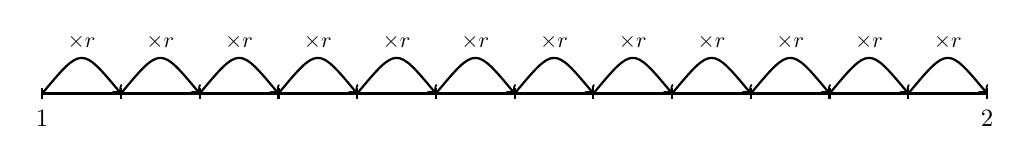
\begin{tikzpicture}
        
        \draw[thick](-6,0) -- (6,0);
        \foreach \x in {-6,-5,-4,-3,-2,-1,0,1,2,3,4,5,6}
            \draw[thick] (\x,2pt) -- (\x,-2pt);
        \node[below,scale=0.9] at (-6,-0.1) {$1$};
        \node[below,scale=0.9] at (6,-0.1) {$2$};

        % Fletxes corbades amb ×r
        \foreach \x in {-6,-5,...,5}
            \draw[->,thick]
            (\x,0) .. controls (\x+0.5,0.6) .. (\x+1,0)
            node[midway,above,scale=0.8] {$\times r$};
    \end{tikzpicture}
    \label{fig:graphic_scale_equal}
\end{figure}
\[
r\times r\times r\times \dotsi \times r=r^{12}=2\implies r=\sqrt[12]{2}
\]
Esta uniformidad tiene una consecuencia fundamental: la distinción entre semitonos diatónicos y cromáticos desaparece en cuanto a su tamaño. Ambos intervalos tienen exactamente la misma razón $r$. Por ejemplo, el semitono diatónico \texttt{\textbf{mi-fa}} y el semitono cromático \texttt{\textbf{do-do}}$\sharp$ son idénticos:
\[
\frac{\texttt{\textbf{fa}}}{\texttt{\textbf{mi}}} = \frac{2^{5/12}}{2^{4/12}} = 2^{1/12} \quad \text{y} \quad \frac{\texttt{\textbf{do}}\sharp}{\texttt{\textbf{do}}} = \frac{2^{1/12}}{2^{0/12}} = 2^{1/12}
\]
Esto garantiza la equivalencia enarmónica (\texttt{\textbf{do}}$\sharp$ $\equiv$ \texttt{\textbf{re}}$\flat$), piedra angular de la música tonal moderna.

Para construir la escala como hemos hecho en otros temperamentos anteriores, podemos razonar que, dado que la escala es igualmente temperada, entonces la suma de dos semitonos sí se correponderá con un tono completo. Por tanto, si un semitono presenta un radio de $\sqrt[12]{2}$, entonces un tono se corresponderá con $(\sqrt[12]{2})^2=\sqrt[6]{2}$. Ahora, iterando esta relación  a partir del $\texttt{\textbf{do}}_4$ por intervalos de 2ª:
\[
\textbf{\texttt{do}$_4$}\equiv1:1
\]
\[
\textbf{\texttt{re}$_4$}\equiv 1\times \sqrt[6]{2}=\sqrt[6]{2}
\]
\[
\textbf{\texttt{mi}$_4$}\equiv \sqrt[6]{2} \times \sqrt[6]{2} =\sqrt[3]{2}
\]
Como entre Mi-Fa hay un semitono, la razón a utilizar es $2^{1/12}$:
\[
\textbf{\texttt{fa}$_4$}\equiv \sqrt[3]{2}\times \sqrt[12]{2} =2^{5/12}
\]
\[
\textbf{\texttt{sol}$_4$}\equiv 2^{5/12}\times 2^{1/6} =2^{7/12}
\]
\[
\textbf{\texttt{la}$_4$}\equiv 2^{7/12}\times 2^{1/6} =2^{9/12}
\]
\[
\textbf{\texttt{si}$_4$}\equiv 2^{9/12}\times 2^{1/6} =2^{11/12}
\]
Nuevamente, se aplica la razón de un único semitono:
\[
\textbf{\texttt{do}$_5$}\equiv 2^{11/12}\times 2^{1/12} =2
\]
En la tabla \ref{tab:scale_12sounds} se pueden observar las relaciones de la escala de Do Mayor temperada.
\begin{table}[h!]
    \centering
    \begin{tabular}{|c||c|c|c|c|c|c|c|c|}
        \hline 
        \textbf{Razón ($a_n/a_{1}$)}&1:1&$\sqrt[6]{2}$:1&$\sqrt[3]{2}$:1&$2^{\frac{5}{12}}$:1&$2^{\frac{7}{12}}$:1&$2^{\frac{9}{12}}$:1&$2^{\frac{11}{12}}$:1&2:1\\
        \hline
        \textbf{Nota}&\texttt{do} & \texttt{re} & \texttt{mi} & \texttt{fa} & \texttt{sol} & \texttt{la} & \texttt{si} & \texttt{do}'  \\
        \hline
    \end{tabular}
    \caption{Escala temperada de \texttt{\textbf{do}}$_4$. Los intervalos sucesivos muestran una estructura regular donde todos los semitonos mesuran igual.}
    \label{tab:scale_12sounds}
\end{table}

En el sistema igualmente temperado, como ya se ha señalado, la uniformidad se logra a costa de la pérdida de pureza de los intervalos consonantes. Este hecho se puede comprobar cuantificando la diferencia entre los intervalos temperados y sus contrapartidas puras.

La quinta temperada ($2^{7/12} \approx 1.4983$) es ligeramente más estrecha que la quinta pura ($3/2 = 1.5$). La diferencia es una desviación apenas perceptible para la mayoría de los oídos. Igualmente en las terceras: la tercera mayor temperada ($2^{4/12} = 2^{1/3} \approx 1.2599$) es notablemente más ancha que la tercera mayor pura de la serie armónica ($5/4 = 1.25$). Estas son algunas de las concesiones que se hacen al adaptar este sistema: se acepta una sonoridad ligeramente más ``brillante'' y tensa en todos los acordes a cambio de la libertad total.

\subsubsection{El semigrupo armónico bien temperado}

Hasta este punto, la justificación del uso del $12$ se ha basado en argumentos aritméticos clásicos (el cierre del círculo de quintas) y en la tradición histórica. Sin embargo, investigaciones recientes, como el trabajo de Bras-Amorós \cite{bras2019tempered}, aportan una perspectiva novedosa que trasciende la acústica clásica: la división en 12 partes es la solución óptima a un problema algebraico de aproximación.

Visto así, la serie armónica física no se contempla solo como un fenómeno acústico, sino como una estructura matemática (un \textit{monoide temperado} de números reales) que evoluciona logarítmicamente. El proceso de establecer un temperamento igual equivale a ``discretizar'' esta realidad continua: se trata de proyectar los armónicos físicos sobre una rejilla de números enteros (las notas del sistema temperado), amplificándolos por un factor $m$ (el número de divisiones de la octava) y redondeando al entero más cercano.

El conjunto de enteros resultante forma un \textit{semigrupo numérico}. Este enfoque establece, además, que no cualquier división $m$ produce un semigrupo que conserve las propiedades esenciales de la música. Bras-Amorós demuestra que para que esta discretización sea consistente, debe satisfacer simultáneamente tres condiciones:

\begin{enumerate}
    \item \textbf{\textit{Compatibilidad de producto:}} La estructura resultante debe respetar la naturaleza logarítmica de la percepción auditiva, donde la suma de intervalos corresponde al producto de frecuencias.
    \item \textbf{\textit{Estructura fractal y áurea:}} El modelo matemático de los armónicos presenta una autosimilitud relacionada con la razón áurea ($\phi$). La escala elegida debe ser capaz de capturar esta naturaleza fractal sin romper la simetría de la bisección de la octava.
    \item \textbf{\textit{Filtrado impar (Odd-filterability):}} Esta es una propiedad acústica crítica. Existen instrumentos, como los tubos cilíndricos cerrados por un extremo (el clarinete), que físicamente solo producen armónicos impares. Un sistema de afinación válido debe ser capaz de modelar algebraicamente este subconjunto de sonidos sin generar inconsistencias en la suma de intervalos.
\end{enumerate}

El resultado principal de dicha investigación prueba que existe un único número de divisiones $m$ capaz de generar un semigrupo numérico que satisfaga estas tres propiedades a la vez. Ese número es, inequívocamente, \textbf{12}.

Si intentáramos dividir la octava en 10, 13 o 18 partes iguales, perderíamos la propiedad de filtrado impar o la coherencia fractal. Al semigrupo generado por la división en 12 se le denomina el \textbf{\textit{semigrupo armónico bien temperado}} (\textit{well-tempered harmonic semigroup}).

Este hallazgo implica que el sistema de 12 semitonos no es meramente una convención cultural o un compromiso de afinación aceptable (``el menos malo''), sino un óptimo matemático. Es la estructura discreta que mejor preserva la compleja riqueza algebraica de la serie armónica continua.

\subsubsection{Conclusión}
Como se ha venido comentando a lo largo del capítulo, la imposición del temperamento igual representa el triunfo del pragmatismo sobre la pureza acústica. Sus numerosas ventajas prácticas --la estandarización de la escritura musical, la libre modulación a cualquier tonalidad y la simplificación en la producción de instrumentos de afinación fija como el piano-- constituyeron los pilares de su adopción generalizada.

Sin embargo, las reticencias históricas que enfrentó por parte de numerosos compositores no fueron infundadas. Sus opositores defendían, con sólidos argumentos acústicos, que no se podía renunciar a la consonancia perfecta ni al carácter único de cada tonalidad. El temperamento igual, al homogeneizar todos los intervalos, sacrificaba la riqueza expresiva de los ``colores'' tonales que definían la estética barroca y clásica, donde la elección entre Do mayor o Fa$\sharp$ mayor conllevaba implicaciones emocionales profundas.

En definitiva, el temperamento igual no es un sistema ``mejor'' o ``peor'' en términos absolutos, sino una solución de compromiso necesaria. Su adopción masiva fue la respuesta a la evolución de la música occidental hacia un lenguaje armónico más flexible. Cierra una búsqueda de dominio de las imperfecciones de la naturaleza acústica pero, al hacerlo, sacrifica una dimensión de expresión musical que los temperamentos anteriores cultivaban con esmero. Su hegemonía es la prueba definitiva de que en la historia de la afinación la solución perfecta no existe: solo existen los equilibrios entre ideales en conflicto.






%{\Large IGUAL AQUÍ PUEDO HABLAR UN POQUILLO DE OTROS SISTEMAS Y EL MICROTONALISMO Y %DEMÄS VAINAS BACANAS ASOCIADAS A LOS TEMPERAMENTOS?} Por ahora queda así

